\documentclass[unicode, notheorems]{beamer}

\mode<presentation>
{
  \usetheme[numbers, totalnumbers]{Madrid}

  \setbeamercovered{transparent}
%
\setbeamertemplate{footline}{%
\hbox{%
\begin{beamercolorbox}[wd=.70\paperwidth,ht=3.25ex,dp=2ex,left,leftskip=2ex]{title in head/foot}%
    \usebeamerfont{title in head/foot}\insertshorttitle{} - \insertshortauthor
\end{beamercolorbox}%
\begin{beamercolorbox}[wd=.20\paperwidth,ht=3.25ex,dp=2ex,center]{date in head/foot}%
    \usebeamerfont{date in head/foot}\insertshortdate{}
\end{beamercolorbox}%
\begin{beamercolorbox}[wd=.10\paperwidth,ht=3.25ex,dp=2ex,right,rightskip=2ex]{date in head/foot}%
    \insertframenumber{} / \inserttotalframenumber
\end{beamercolorbox}}%
}

}
\usepackage{graphicx}
\usepackage{tikz}
%\usepackage{unicode-math}
%\setmathfont{XITS Math}
%\setmathfont[version=setB,StylisticSet=1]{XITS Math}
\usepackage{mathrsfs}

\usepackage[T2A]{fontenc}
\usepackage[utf8]{inputenc}
\usepackage[russian]{babel}
\usepackage{amsthm}
\usepackage{amsfonts}
\newcommand{\R}{\mathbb{R}}
\newcommand{\N}{\mathbb{N}}
\newcommand{\E}{\mathbb{E}}
\newcommand{\D}{\mathbb{D}}
\newcommand{\T}{\mathrm{T}}
\usepackage{amsfonts}
\usepackage{amsmath}
\usepackage{multicol}


\usepackage[T2A]{fontenc}
\ifpdf\usepackage{epstopdf}\fi

\newtheorem{theorem}{Теорема}
\newtheorem{example}{Example}
\newtheorem{definition}{Определение}
\newcommand{\scal}[2]{\left\langle #1,#2 \right\rangle}

\title{Регуляризация в регрессии}

\author{Ширинкина Дарья Андреевна, гр. 622}
\institute[СПбГУ]{Санкт-Петербургский государственный университет \\
Математико-механический факультет \\
    Статистическое моделирование
    
    \vspace{0.4cm}

    \vspace{0.3cm}
}
\date{
    Санкт-Петербург\\
    2017г.
}

\subject{Beamer}

\begin{document}

\begin{frame}
    \titlepage%3-5/diploma/2017m/index.html
\end{frame}



\begin{frame}
\frametitle{Задача}
\textbf{Пусть}
\begin{itemize}
\item $x_1, \ldots, x_n \in \R^p$ --- независимые одинаково распределенные случайные величины; 
\item $X = [X_1, \ldots, X_p]$, где $X_i = (x_{1i}, \ldots, x_{ni})^{\T}$, $i = 1, \ldots, p$.
\end{itemize}
\vspace{0.5cm}
Предполагаем существование неизвестной $f$ такой, что 
\[y_i = f(x_i) + \varepsilon_i,\]

где 
\begin{itemize}
\item $Y = (y_1, \ldots, y_n)^{\T} \in \R^n$;
\item $\varepsilon = (\varepsilon_1, \ldots, \varepsilon_n)$ --- независимые случайные величины;
\item $\varepsilon_i$ и $x_j$ независимы для $\forall i,j$;
\item $\E\varepsilon_i = 0$, $i = 1, \ldots, n$ и $\E\varepsilon_i^2 = \sigma^2$.
\end{itemize}

\vspace{0.5cm}
\textbf{Задача: } Оценить функцию $f$.
\vspace{0.3cm}

\end{frame}


\begin{frame}
\frametitle{Обозначения}

\textbf{Обучающая выборка:}
\begin{itemize}
\item $x_1, \ldots, x_n$ --- выборка, участвующая в оценке функции $f$ (обучающая выборка);
\item $y_i = f(x_i) + \varepsilon_i$, $i = 1, \ldots, n$.  
\end{itemize} 
\vspace{1cm}

\textbf{Тестовая выборка:}
\begin{itemize}
\item $x_1', \ldots, x_k'$ --- выборка, по которой оценивается качество оценки функции $f$ (тестовая выборка);
\item $y_i' = f(x_i') + \varepsilon_i'$, $i = 1, \ldots, k$.  
\end{itemize} 
\end{frame}



\begin{frame}
\frametitle{Модель}

Считаем, что $Y = (y_1, \ldots, y_n)^{\T}$ и $X$ --- центрированы. %$\E x_i = 0$.
\vspace{0.8cm}

\textbf{Модель многомерной линейной регрессии:}

\[y_i = f(x_i, \beta) + \varepsilon_i = \sum_{j=1}^p \beta_j x_{ij} + \varepsilon_i.\]

\textbf{Задача минимизации: } 

\[\mathrm{MSE}_{\mathrm{training}} = \frac{1}{n}\sum_{i=1}^n(y_i - \sum_{j=1}^p \beta_j x_{ij})^2 \rightarrow \min_{\beta}.\]
\vspace{0.6cm}

\textbf{Решение МНК: } $\hat{\beta} = (X^{\T}X)^{-1} X^{T}Y.$

\end{frame}



\begin{frame}
\frametitle{Проблема}

Насколько хорошо предсказывает $\hat{f}(x) = \sum_{i=1}^p \hat{\beta}_i x$?

\vspace{0.5cm}

\textbf{Проблема:} минимизируем $\mathrm{MSE}_{\mathrm{training}}$, но хотим минимизировать 

\[\mathrm{MSE}_{\mathrm{test}} = \frac{1}{n}\sum_{i=1}^n(y_i' - \sum_{j=1}^p \beta_j x_{ij}')^2.\]
\vspace{0.3cm}

\begin{itemize}
\item Нет гарантии, что минимум $\mathrm{MSE}_{\mathrm{training}}$ будет соответствовать минимуму $\mathrm{MSE}_{\mathrm{test}}$.
\item Когда $\mathrm{MSE}_{\mathrm{test}} \gg \mathrm{MSE}_{\mathrm{training}}  $, говорят, что происходит переобучение.
\end{itemize}



\end{frame}

\begin{frame}
\frametitle{Проблема}

Пусть
\begin{itemize}
\item $x_i'$ --- реализация случайной величина из тестовой выборки;
\item $y_i' = f(x_i') + \varepsilon_i'$ --- известное значение.
\end{itemize}

\[\E(y_i' - \hat{f}(x_i'))^2 = Var(\hat{f}(x_i')) + (Bias(\hat{f}(x_i')))^2 + Var(\varepsilon_i').\]

\vspace{0.8cm}
\begin{itemize}
\item Как правило, при увеличении сложности метода (увеличение числа параметров) дисперсия будет увеличиваться, а смещение будет уменьшаться.
\item Введение небольшого смещения в оценке может привести к значительному уменьшению дисперсии и тем самым уменьшению $\mathrm{MSE}_{\mathrm{test}}$.  
\end{itemize}


\end{frame}




\begin{frame}
\frametitle{Регуляризация}

\textbf{Регуляризация:} вводим ограничения на коэффициенты $\beta$.

\vspace{0.8cm}
Для чего используем регуляризацию:
\begin{itemize}
\item можем уменьшить дисперсию оценки за счет введения смещения и тем самым уменьшить $\mathrm{MSE}_{\mathrm{test}}$ (особенно, когда $p >n$);
\item можем производить отбор значимых признаков, делая коэффициенты при них равными нулю.
\end{itemize}


\end{frame}


\begin{frame}
\frametitle{Гребневая регрессия}

Задача минимизации:

\[\sum_{i=1}^n(y_i - \sum_{j=1}^p \beta_j x_{ij})^2  + \lambda \sum_{j = 1}^p \beta_j^2 \rightarrow \min_{\beta},\]

где $\lambda \geq 0$ --- неотрицательный параметр регуляризации (tuning parameter).

\begin{itemize}
\item $\lambda\sum_{j = 1}^p \beta_j^2$ мало, когда $\beta_1, \ldots, \beta_p$ близки к нулю.
\item Когда $\lambda = 0$, то гребневая регрессия совпадает с обычной регрессией, но при $\lambda \rightarrow \infty$ коэффициенты регрессии стремятся к нулю.

\item Необходимо выбрать хорошее значение $\lambda$.
\end{itemize}


\end{frame}




\begin{frame}
\frametitle{Способ решения оптимизационной задачи}

Модифицированное МНК решение гребневой регрессии:
\[\hat{\beta}_{\lambda}^{R} = (X^{\mathrm{T}}X+ \lambda I_p)^{-1} X^{\mathrm{T}}Y.\]

Решение через сингулярное разложение, где $X = VDU^{\T}$:

\begin{itemize}
\item \textbf{МНК}
\[\hat{\beta} = \sum_{j=1}^p \frac{1}{\sqrt{\lambda_j}} U_j(V_j^{\T}Y);\]
\item \textbf{МНК гребневой регрессии }
\[\hat{\beta}_{\lambda}^{R} = U(D^2 + \lambda I_p)^{-1}DV^{\T}y = \sum_{j=1}^p \frac{\sqrt{\lambda_j}}{\lambda_j + \lambda} U_j(V_j^{\T}Y).\]

\end{itemize}

С помощью сингулярного разложения можно быстро выбирать параметр $\lambda$.

\begin{frame}
\frametitle{Выбор параметра регуляризации}

Как выбрать параметр $\lambda$:
\begin{itemize}
\item выбираем сетку значений $\lambda$;
\item вычисляем ошибку кросс-проверки для каждого значения $\lambda$;
\item выбираем $\lambda$ с наименьшим значением ошибки кросс-проверки;
\item перестраиваем модель со всеми наблюдениями с выбранным значением $\lambda$.
\end{itemize}


\end{frame}





\begin{frame}
\frametitle{Вероятностная интерпретация} 

\begin{itemize}
\item $\beta = (\beta_1, \ldots, \beta_p)^{\T}$ имеет априорное распределение $p(\beta)$;
\item $f(Y|X,\beta)$ --- функция правдоподобия исходных данных. 
\end{itemize}

\vspace{0.3cm}
При фиксированном $X$ апостериорное распределение $p(\beta|X,Y)$ пропорционально 
\[f(Y|X,\beta)p(\beta|X) = f(Y|X,\beta)p(\beta).\]

Предполагая, что 
\begin{enumerate}
\item линейная модель имеет независимые и нормально распределенные ошибки; 
\item $p(\beta) = \prod_{j = 1}^p g(\beta_j)$ для некоторой плотности $g$.
\end{enumerate}

\vspace{0.5cm}
Если $g$ --- плотность $N(0,\lambda)$, то  оценка апостериорного максимума $\beta$ совпадает с решением гребневой регрессии.

\end{frame}


\begin{frame}
\frametitle{Смещение оценки}

Пусть $X^{\T}X = \Sigma$ и $Y = (y_1, \ldots, y_n)^{\T}$.

Оценка гребневой регрессии через МНК оценку:

\begin{align*}
\hat{\beta}_{\lambda}^R = (I_p + \lambda \Sigma^{-1})\hat{\beta}.  
\end{align*}

Оценка гребневой регрессии имеет смещение:

\begin{align*}
\E\hat{\beta}_{\lambda}^{R} &= \E[(I_p + \lambda \Sigma^{-1})\hat{\beta}] = \\
	&= (I_p + \lambda \Sigma^{-1})\beta.
\end{align*} 

Если $\lambda = 0$, то оценка гребневой регрессии не имеет смещения.
\end{frame}





\begin{frame}
\frametitle{Свойства}

\begin{itemize}
\item Оценки МНК инварианты относительно умножения признака на константу, то есть значение $f(x_j)\hat{\beta_j}$ не зависит от масштаба $j$-го признака. 
\item Инвариант относительно масштаба теряется в случае гребневой регрессии, оценки МНК гребневой регрессии могут сильно измениться при умножении заданного признака на константу.
\end{itemize}

\vspace{0.3cm}
\textbf{Вывод:} гребневую регрессию нужно использовать после стандартизации признаков.
\vspace{0.8cm}

\textbf{Проблема:} 
\begin{itemize}
\item в конечную модель входят все начальные признаки;
\item если признаков много, то усложняется интерпретация.
\end{itemize}

\end{frame}


%%%%%%%%%%%%%%%%%%%%%%%%%%%%%%%%%%%%%%%%%


\begin{frame}
\frametitle{Лассо регрессия}


Задача минимизации:


\[\sum_{i=1}^n(y_i - \sum_{j=1}^p \beta_j x_{ij})^2 + \lambda \sum_{j = 1}^p |\beta_j| \rightarrow \min_{\beta},\]

где $\lambda \geq 0$ --- неотрицательный параметр регуляризации (tuning parameter).

\begin{itemize}
\item Как и в гребневой регрессии $\lambda \sum_{j = 1}^p |\beta_j|$ мало, когда $\beta_1, \ldots, \beta_p$ близки к нулю.
\item При увеличении параметра $\lambda$ некоторые коэффициенты регрессии становятся равными нулю.
\item Как и в гребневой регрессии необходимо выбрать хорошее значение $\lambda$.
\end{itemize}

\end{frame}







\begin{frame}
\frametitle{Способ решения оптимизационной задачи}
Задача:

\[\sum_{i=1}^n(y_i - \sum_{j=1}^p \beta_j x_{ij})^2 + \lambda \sum_{j = 1}^p |\beta_j| \rightarrow \min_{\beta}\]

эквивалента задаче минимизации с ограничением:

\begin{align*}
\sum_{i=1}^n(y_i - \sum_{j=1}^p \beta_j x_{ij})^2 \rightarrow \min_{\beta}, \qquad  \sum_{j = 1}^p |\beta_j| \leq s,
\end{align*}
где параметру $\lambda$ соответствует параметр $s$.

\begin{itemize}
\item Чем меньше $s$, тем больше нулевых значений коэффициентов $\beta$.
\item Значение параметра $\lambda$ выбирается как в гребневой регрессии с помощью кросс-проверки.
\end{itemize}

 

\end{frame}

\begin{frame}
\frametitle{Вероятностная интерпретация}

\begin{itemize}
\item $\beta = (\beta_1, \ldots, \beta_p)^{\T}$ имеет априорное распределение $p(\beta)$;
\item $f(Y|X,\beta)$ --- функция правдоподобия исходных данных. 
\end{itemize}

\vspace{0.3cm}
При фиксированном $X$ апостериорное распределение $p(\beta|X,Y)$ пропорционально 
\[f(Y|X,\beta)p(\beta|X) = f(Y|X,\beta)p(\beta).\]

Предполагая, что 
\begin{enumerate}
\item линейная модель имеет независимые и нормально распределенные ошибки; 
\item $p(\beta) = \prod_{j = 1}^p g(\beta_j)$ для некоторой плотности $g$.
\end{enumerate}

\vspace{0.5cm}
Если $g$ --- плотность распределения Лапласса с нулевым средним и параметром масштаба $\lambda$, то оценка апостериорного максимума $\beta$ является решением Лассо. 


\end{frame}


\begin{frame}
\frametitle{Свойства}
Почему Лассо обнуляет коэффициенты.

\begin{figure}
\center{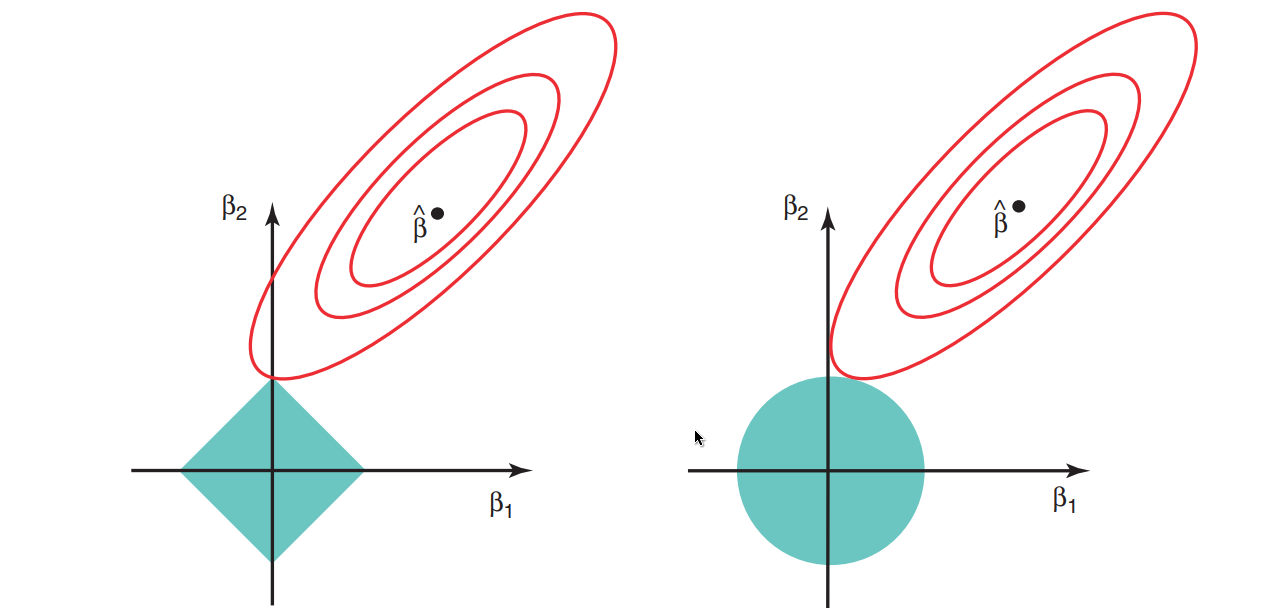
\includegraphics[width=1\linewidth]{Lasso_and_ridge.png}}
\caption{Границы ошибки $\sum_{i=1}^n(y_i - \sum_{j=1}^p \beta_j x_{ij})^2$ и ограничений  $\sum_{j = 1}^p |\beta_j| \leq s$ для Лассо (слева) и $\sum_{j = 1}^p \beta_j^2 \leq s$ для гребневой регрессии (справа).}
\end{figure}

\end{frame}


\begin{frame}
\frametitle{Сравнение гребневой регрессии и Лассо}
Рассмотрим простой случай, когда $n = p$ и $X$ --- диагональная матрица с $1$ на диагонали.

\textbf{МНК:}

\[\sum_{j =1}^p (y_j - \beta_j)^2.\]

\textbf{Решение гребневой регрессии:}
\[\hat{\beta}_{\lambda}^R = \frac{y_j}{1 + \lambda}.\]

\textbf{Решение Лассо:}
\begin{equation*}
\hat{\beta}_{\lambda}^L = 
 \begin{cases}
   y_j - \lambda/2, & \qquad y_j > \lambda/2\\
   y_j + \lambda/2, & \qquad y_j < -\lambda/2 \\
   0, & \qquad |y_j| \leq \lambda/2.
 \end{cases}
\end{equation*}



\end{frame}


\begin{frame}
\frametitle{Сравнение гребневой регрессии и Лассо}
\vspace{-0.3cm}

\begin{figure}
\center{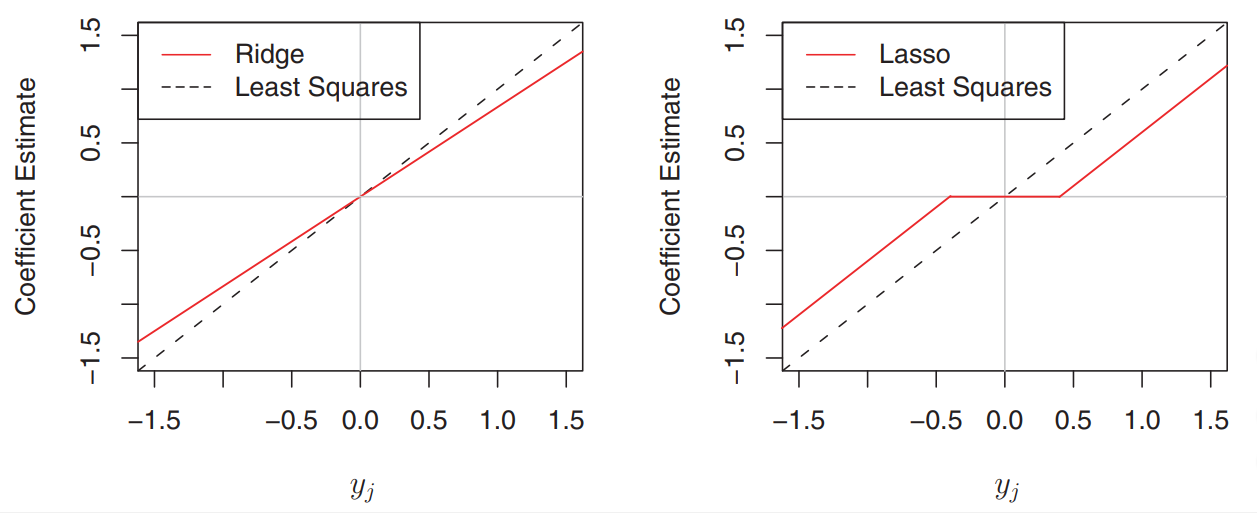
\includegraphics[width=1\linewidth]{compare.png}}

\end{figure}
\vspace{-0.3cm}

\begin{itemize}
\item Гребневая регрессия уменьшает каждый коэффициент с равной пропорцией; 
\item Лассо уменьшает значения коэффициентов на одинаковое значение;
\item В Лассо, если коэффициент по модулю меньше $\lambda/2$, то его значение становится равным нулю.
\end{itemize}

\end{frame}

\begin{frame}
\frametitle{Сравнение гребневой регрессии и Лассо}

Нельзя выделить ни одну из моделей (Лассо или гребневая регрессия) как лучшую.

\vspace{0.8cm}
Можно ожидать, что 
\begin{itemize}
\item Лассо будет иметь ошибку меньше, когда в модели мало значимых признаков (коэффициенты при таких признаках будут равны нулю);
\item Гребневая регрессия будет иметь ошибку меньше, когда $Y$ будет зависеть от признаков, которые имеют примерно равную значимость. 
\end{itemize}


\vspace{0.8cm}
С помощью кросс-проверки можно определить какой подход лучше.

\end{frame}

\end{document}